\documentclass[11pt]{article}

\usepackage[margin=1in]{geometry}
\usepackage{amsmath,amssymb,amsthm}
\usepackage{booktabs}
\usepackage{enumitem}
\usepackage{flafter}
\usepackage{graphicx}
\usepackage{placeins}
\usepackage[hidelinks]{hyperref}

\setlist[itemize]{leftmargin=1.4em}
\setlist[enumerate]{leftmargin=1.6em}

\newcommand{\KL}{D}
\newcommand{\E}{\mathbb{E}}
\newcommand{\Nseq}{N}
\newcommand{\model}{\mathcal{M}_{d,L}}
\newcommand{\cstar}{c^\star}
\newtheorem{proposition}{Proposition}
\newtheorem{remark}{Remark}

\title{A Product Model for Sources with Memory}
\author{}
\date{\today}

\begin{document}

\title{Earlier experiments: a record}
\date{split out 3 August 2026}
\maketitle

\noindent This file preserves exploratory experiments that
preceded the pairwise program: the state-map families, the
context trees, the lag profile, the pooled lags, the
comparison section, and the joint-pair diagnostic.  The
numbers were computed with the pre-August machinery and have
not been re-verified under the corrected evaluator; treat
them as directional.  Some references (rendered as ??) point
into the main paper.  Ideas here are expected to resurface;
nothing is endorsed by inclusion.

\section{Families of state maps}
\label{sec:states}

\emph{Representation.  From here to
Section~\ref{sec:comparison} the symbol is a \texttt{text8} word:
\texttt{text8} split on spaces, the space folded into the word,
$253{,}854$ types.  This is a third alphabet, distinct from the two of
Section~\ref{sec:sources}, and it applies to \texttt{text8} alone, since
\texttt{enwik8} and \texttt{enwik9} are raw markup with nothing to
split on.  Its figures are therefore not comparable with
Tables~\ref{tab:memoryless} and~\ref{tab:firstorder}: a different
alphabet over a different file.  What the sections below establish is
the behaviour of the constructions, not a benchmark position.}

This section records the general program that fixes the design
principle for everything that follows.

A memory model is a \emph{state map} $\sigma$ compressing the past into a
state, $s_t=\sigma(x^{t-1})$, followed by the estimation machinery on
$(\text{state},\text{next token})$ pairs.  The quality of $\sigma$ at a
given data budget decomposes into two terms that move in opposite
directions:
\begin{itemize}
\item the \emph{ceiling} $\hat H(X_{t+1}\,|\,S)$ --- the best conditional
  log-loss any predictor built on these states can reach --- which falls as
  states become finer (last token, last two tokens, \dots); and
\item the \emph{learning cost} --- the redundancy paid to estimate one
  conditional per state --- which grows with the number of states and is
  governed, as in the scaling analysis of \cite{layered2026}, by the rate
  at which new $(\text{state},\text{successor})$ pairs are discovered.
\end{itemize}
Total codelength is the sum, and ``finding good states'' means optimizing
this sum.  Both terms are computable in our framework: the ceiling
empirically, the learning cost exactly through the regret calculus.
Section~5.4 of \cite{layered2026} exhibits the trade-off in miniature (the
interior optimum in the number of split contexts); here it becomes the main
object of study.

The design principle is to treat memory \emph{exactly as depth is treated}.
The depth-averaged predictor does not select a depth: it averages the
mixtures of all depths $L \le L_{\max}$ and pays at most
$(\log_2 L_{\max})/n$ per token for not knowing the right depth in
advance, a price that vanishes as $n$ grows.  Correspondingly, we
do not intend to select a single state map: we define a \emph{nested
family} $\sigma_1 \preceq \sigma_2 \preceq \cdots \preceq \sigma_M$ of
state maps of increasing memory (each refining the last), place a prior
over the family, and use the single coherent Bayesian mixture
\begin{equation}
\label{eq:state-average}
  Q(x^n) \;=\; \sum_{m=1}^{M} \pi_m\, Q^{(\sigma_m)}(x^n),
\end{equation}
where $Q^{(\sigma_m)}$ is the (depth-averaged) layered predictor built on
the states of $\sigma_m$.  The data then \emph{selects the effective
memory} through the posterior over $m$, just as it now selects the
effective depth, at a model-selection price of at most $(\log_2 M)/n$ bits
per token.  Memory is then handled in the same way as depth: not one
$\sigma$ for all sources, but one prior whose mass is spread over all the
state maps the family contains.

Concrete instances of the family, in increasing order of generality:
(i) the top-$K$ sequence of Appendix~\ref{sec:pairs}, i.e.\ the last token
bucketed by frequency, a first coarse compression of the past into a
state; (ii) variable-length suffixes of the past, i.e.\ context trees,
where averaging over the family recovers the structure of context-tree
weighting but with layered mixtures at the leaves in place of KT
estimators (the layered prior dominates KT on large alphabets
\cite{layered2026}); (iii) states obtained by \emph{clustering} last
tokens by similarity of their successor distributions (merge states that
predict alike, sweep the cluster count), the first family whose members
are constructed from the data rather than fixed in advance;
(iv) learned continuous state maps, which connect this program to the
architecture-as-prior view of \cite{layered2026}, Section~6: a state map
is an architecture, and its design determines where the prior puts its
mass over predictors.  The limiting case --- states defined by ``two
pasts are equivalent iff they induce the same conditional law of the
future'' (causal states) --- cannot be learned directly; it describes
what the constructions above approximate.

Orthogonal to the choice of states is the question of \emph{coupling}:
whether the per-state conditionals are estimated independently (the
share-nothing construction of \cite{layered2026}, Section~5.4) or jointly,
as in Appendix~\ref{sec:pairs}, where the prior on the joint pair
distribution lets every row's smoothing be informed by the count
statistics of all rows.  The two axes --- what the states are, and whether
they share statistical strength --- should be varied separately; the
comparison of joint-coupled versus share-nothing estimation at identical
states isolates the value of coupling.

\subsection{First instance: the context-partition family}
\label{sec:state-family}

The simplest implementation of the program is the following
(\texttt{scripts/state\_family\_experiment.py}).  Fix the emission
vocabulary to the top $K$ tokens plus $\langle\mathrm{unk}\rangle$
($V=K{+}1$).  The family members are the state maps
\[
  \sigma_M:\quad
  s_t \;=\;
  \begin{cases}
    x_{t-1} & \text{if } x_{t-1} \text{ is among the top } M
      \text{ tokens},\\
    \langle\mathrm{other}\rangle & \text{else},
  \end{cases}
  \qquad M \in \{0, 1, 2, 4, \dots, V\},
\]
nested and log-spaced; $\sigma_0$ has a single state and \emph{is} the
memoryless predictor of Section~\ref{sec:text8}, so the family contains
``no memory'' as its coarsest member.  Each member is scored by the
sequential share-nothing code: conditioned on the state the successor
sub-sequence is exchangeable, so
$Q^{(\sigma_M)}(x^n)=\prod_{s} q^{\mathrm{avg}}\bigl(\text{successor
profile of } s\bigr)$, every factor a per-state depth-averaged layered
mixture evaluated exactly from counts (this is the construction of
\cite{layered2026}, Section~5.4, rebuilt from the validated port).  The
family average is the uniform mixture \eqref{eq:state-average}; all
members share one emission alphabet and hence one moment-table cache, so
the whole family costs little more than its finest member.

Three predictions are checked.  (i) The member codelengths trace an
interior optimum in $M$: coarse members pay in ceiling, fine members pay
in learning cost, and the minimizer is the data-determined effective
memory.  (ii) The posterior over $M$ concentrates at that optimum.
(iii) The family mixture tracks the best member to within
$(\log_2 |\mathrm{grid}|)/n$ bits/token, so memory-averaging, like
depth-averaging, costs almost nothing.  The member codelengths are those
of sequential codes; comparing the best member with the in-sample
plug-in value of Table~\ref{tab:pairs} measures the additional cost of
estimating the conditionals as the data arrive rather than from the
whole corpus.

\paragraph{Order-two extension (implemented).}
The family need not stop at the previous token.  With the same fixed
emission vocabulary, define product states with \emph{asymmetric
resolution},
\[
  \sigma_{M_1,M_2}:\quad
  s_t \;=\; \bigl(b_{M_1}(x_{t-1}),\, b_{M_2}(x_{t-2})\bigr),
\]
where $b_M$ keeps a token if among the top $M$ and buckets it otherwise
($b_0$ buckets everything).  The grid over $(M_1, M_2)$ contains the
first-order family as its $M_2=0$ slice and memoryless as $(0,0)$; all
members code $x_3,\dots,x_n$ over the same alphabet and are therefore
mixable exactly as before
(\texttt{scripts/product\_family\_experiment.py}).  The posterior over
the grid is now a measurement of how predictive resolution should be
\emph{split across distances into the past} at a given data budget.
Computationally the member count is reduced by a global deduplication:
rare contexts overwhelmingly share identical tiny successor profiles, so
the $\sim 2\cdot 10^5$ states of a ten-member grid on full \texttt{text8}
collapse to $\sim 2.7\cdot 10^4$ unique profiles, each evaluated once.

\subsubsection*{The first order-two experiment}
At $V=1{,}024$ the family uses the
ten-member grid
\[
  \{(0,0)\} \;\cup\; \{(M,0): M = 64, 256, 1024\}
  \;\cup\; \{(1024, M_2): M_2 = 4, 16, 64, 256\}
  \;\cup\; \{(256,16), (64,64)\},
\]
designed to ask three questions at once.  (i)~The $M_2=0$ slice anchors
the grid to the first-order family of Table~\ref{tab:state-family}
(values shift microscopically because all members now code
$x_3,\dots,x_n$).  (ii)~The arm $(1024, M_2)$ with growing $M_2$ asks:
\emph{on top of full one-back resolution, what is progressively finer
resolution of the token two positions back worth, and when does it stop
paying?}
This is the second axis of the boundary-versus-interior question that
the first-order family, monotone up to $M=V$, left open.
(iii)~The members $(256,16)$ and $(64,64)$ hold the number of states
roughly comparable to $(1024,0)$ ($\sim$1--4k states) while splitting
resolution differently across the two distances: \emph{given a budget of
states, should they resolve the recent past finely, or spread across
more history?}  The posterior over the grid answers all three; the
outcomes of interest are whether the second axis, too, is monotone up to
the boundary at this $n$ (pushing the effective-memory frontier beyond
order one entirely), and, if not, where the interior split lands.

\begin{table}[ht]
\centering
\begin{tabular}{rrrrr}
\toprule
$M_1$ & $M_2$ & states obs. & bits/token & posterior \\
\midrule
    0 &    0 &        1 & 6.0636 & $0$ \\
   64 &    0 &       65 & 5.3773 & $0$ \\
  256 &    0 &      257 & 5.2144 & $0$ \\
 1024 &    0 &    1{,}024 & 5.0564 & $0$ \\
 1024 &    4 &    4{,}989 & 5.0395 & $0$ \\
 1024 &   16 &   15{,}950 & 5.0138 & $0$ \\
 1024 &   64 &   47{,}687 & \textbf{5.0104} & $1.0$ \\
 1024 &  256 &  127{,}078 & 5.0419 & $0$ \\
  256 &   16 &    4{,}251 & 5.1411 & $0$ \\
   64 &   64 &    3{,}891 & 5.2443 & $0$ \\
\bottomrule
\end{tabular}
\caption{Order-two product-state family on full \texttt{text8}
  ($V=1{,}024$, sequential per-state codes, all members coding
  $x_3,\dots,x_n$; family mixture $5.0104$ bits/token $=$ best member).
  Along the arm $(1024, M_2)$ the codelength decreases through
  $M_2 = 4, 16$ to its minimum at $M_2^\star = 64$ and increases again
  at $M_2 = 256$: resolution $64$ on the token two positions back
  reduces the codelength by $0.046$ bits/token relative to $(1024,0)$,
  while finer two-back resolution costs more to learn than it gains.
  This is the first family in the sequence whose optimum lies in the
  interior of the grid, and the posterior concentrates on it.  The
  constant-budget members answer the split question: at roughly equal
  state counts, $(1024,4)$ gives a shorter codelength than $(256,16)$,
  which gives a shorter codelength than $(64,64)$; resolution on the
  most recent token is worth more than resolution further back.  Along
  the first-order axis (Table~\ref{tab:state-family}) the optimum was
  always at the boundary; the trade-off appears once memory extends
  further back.}
\label{tab:product-family}
\end{table}

\begin{table}[ht]
\centering
\begin{tabular}{rrrrr}
\toprule
$M_1$ & $M_2$ & states obs. & bits/token & posterior \\
\midrule
    0 &    0 &        1 & 8.0523 & $0$ \\
  256 &    0 &      257 & 7.0742 & $0$ \\
 1024 &    0 &    1{,}025 & 6.8776 & $0$ \\
 4096 &    0 &    4{,}096 & \textbf{6.7132} & $1.0$ \\
 4096 &   16 &   56{,}096 & 6.7855 & $0$ \\
 4096 &   64 &  147{,}784 & 6.8592 & $0$ \\
 4096 &  256 &  318{,}201 & 6.9601 & $0$ \\
 4096 & 1024 &  640{,}407 & 7.1486 & $0$ \\
 1024 &   64 &   47{,}752 & 6.8777 & $0$ \\
 1024 &  256 &  127{,}335 & 6.9317 & $0$ \\
\bottomrule
\end{tabular}
\caption{The same family at $V=4{,}096$ (family mixture $6.7132$
  bits/token $=$ best member): the optimum returns to the first-order
  boundary.  Every allocation of two-back resolution now increases the
  codelength --- $(4096, 16)$ already costs $0.07$ bits/token --- and
  the two-back resolution that was worth $0.046$ bits/token at
  $V=1{,}024$ is worth nothing here: $(1024,64)$ equals $(1024,0)$ to
  four decimals.  Together with Table~\ref{tab:product-family} this
  shows that the location of the optimum is not monotone in $V$ at
  fixed $n$: enlarging the emission alphabet raises every state's
  estimation cost, and the data budget that at $V=1{,}024$ left a
  surplus for order-two structure is at $V=4{,}096$ fully consumed by
  order one.  The result also shows a limitation of \emph{uniform}
  product states: the same two-back resolution is applied after every
  first-order state, frequent or rare.  A family whose members can
  allocate depth per context is the subject of
  Section~\ref{sec:context-tree}.}
\label{tab:product-family-4096}
\end{table}

\paragraph{Scaling sequence.}
As with the pair diagnostic (Appendix~\ref{sec:pairs}), the same code is run at a sequence of
scales: (1) $V=64$, $n=10^6$ (small test run); (2) $V=256$, full
\texttt{text8} (laptop); (3) $V=1{,}024$ and $V=4{,}096$, full corpus
(laptop, overnight), where the fine members are sparsely observed;
(4) $V$ at the full vocabulary and richer families (order-two states on
the bucketed alphabet, clustered states), on the cluster.  The
quantities tracked are the location $M^\star$ of the optimum as a
function of $(V, n)$, and the margin between the family mixture and
both its $M=0$ member (the value of memory) and the in-sample plug-in
value of Table~\ref{tab:pairs} (the cost of sequential estimation).

\begin{table}[ht]
\centering
\begin{tabular}{rrrrrrr}
\toprule
$V$ & $n$ & $\hat H(x'|x)$ & $M^\star$ & best member & family & $M=0$ member \\
\midrule
 64 & $10^6$        & 2.753 &  64 (bd.) & 2.7644 & 2.7644 & 3.2573 \\
256 & $1.7\cdot10^7$ & 3.709 & 256 (bd.) & 3.7198 & 3.7198 & 4.4234 \\
1{,}024 & $1.7\cdot10^7$ & 4.979 & 1024 (bd.) & 5.0564 & 5.0564 & 6.0636 \\
4{,}096 & $1.7\cdot10^7$ & 6.338 & 4096 (bd.) & 6.7132 & 6.7132 & 8.0523 \\
\bottomrule
\end{tabular}
\caption{Context-partition family: location $M^\star$ of the posterior
  mode, best-member and family-mixture codelengths (bits/token,
  sequential codes), and the memoryless member, per scale $(V,n)$.  At
  all scales run so far the optimum sits at the \emph{boundary} (bd.):
  the member curve falls monotonically in $M$, the posterior puts mass
  $1.0$ on the finest member, and the family mixture equals the best
  member to four decimals, as the $(\log_2|\mathrm{grid}|)/n$ bound
  requires.  The boundary optimum persists even at $V=1{,}024$, where
  $71\%$ of the pair alphabet is unseen: a thousand share-nothing
  states are still worth their learning cost at $n=1.7\cdot10^7$; with
  the layered per-state prior, the cost of adding rare states is small
  enough that refining pays at every scale tried.  The sequential code
  obtains $98.6\%$ ($V=256$), $92.9\%$ ($V=1{,}024$), and $78.2\%$
  ($V=4{,}096$) of the in-sample memory value
  $\hat H_1 - \hat H(x'|x)$; its excess over the plug-in value of
  Table~\ref{tab:pairs} grows $0.0105 \to 0.0771 \to 0.3756$
  bits/token.  An interior optimum still does not appear: even four
  thousand share-nothing states, the rarest observed only dozens of
  times, each reduce the codelength by more than their learning cost at
  $n=1.7\cdot10^7$.  For last-token state maps at this corpus size the
  optimum lies at or beyond the full vocabulary; an interior optimum
  first appears when the family is extended to order two
  (Table~\ref{tab:product-family}).}
\label{tab:state-family}
\end{table}

\subsubsection*{The endpoints at the full vocabulary}
\label{sec:state-family-endpoints}
The same family evaluated at the full vocabulary
($V = 253{,}855$: every observed type plus an unused bucket symbol;
grid endpoints $M = 0$ and $M = V$; $253{,}854$ observed states,
$4{,}146{,}848$ distinct pairs deduplicating to $26{,}164$ unique
profiles; $106$ minutes) extends Table~\ref{tab:state-family} by one
scale:
\[
  M{=}0:\ 10.8942, \qquad M{=}V:\ \mathbf{10.0909}
  \quad\text{bits/token},
\]
with posterior mass $1.0$ on $M = V$ and the family mixture equal to
the best member plus the one-bit grid prior.  (The $M{=}0$ member
reproduces the Section~\ref{sec:text8} memoryless code; the small
difference from $10.8952$ is the alphabet, $253{,}855$ against
$2^{18}$.)  The boundary ordering persists: even $253{,}854$
share-nothing states, most observed a handful of times, are jointly
worth their learning cost.  But the sequential code now captures only
$0.8033$ of the in-sample memory value
$\hat H_1 - \hat H(x'|x) = 10.8563 - 7.2863 = 3.5700$ bits/token ---
$22.5\%$, continuing the fall $98.6\% \to 92.9\% \to 78.2\%$ of
Table~\ref{tab:state-family} --- and the excess over the plug-in
conditional entropy is now $2.8046$ bits/token.  At this scale the
complete first-order map is a blunt instrument: it buys every word its
own successor row, including hundreds of thousands of rows that can
never repay their cost individually and are carried only by the
aggregate.

\subsubsection*{The interior optimum}
The intermediate members settle where the resolution should stop
(Table~\ref{tab:interior-m}; cluster run, $34$ minutes).  For the
first time in the first-order family the optimum is \emph{interior}:
$M^\star = 4{,}096$, i.e.\ the code that gives the $4{,}096$ most
frequent words their own successor row and pools the remaining
$249{,}758$ words into one shared backoff row is the best member ---
better than the complete map by $0.3083$ bits/token and better than
every neighbor on the grid, with posterior mass $1.0$.  The boundary
optima of Table~\ref{tab:state-family} were a small-$V$ phenomenon:
once the vocabulary is no longer capped, the data can finally express
where refinement stops paying, and it stops at a few thousand words.

\begin{table}[ht]
\centering
\begin{tabular}{rrr}
\toprule
$M$ & states obs. & bits/token \\
\midrule
      0 &        1 & 10.8942 \\
 1{,}024 &  1{,}025 &  9.8316 \\
 4{,}096 &  4{,}097 & \textbf{9.7826} \\
16{,}384 & 16{,}385 &  9.8682 \\
65{,}536 & 65{,}537 & 10.0060 \\
253{,}854 & 253{,}854 & 10.0909 \\
\bottomrule
\end{tabular}
\caption{The first-order family at the full emission vocabulary
  ($V = 253{,}855$), members $\sigma_M$: top-$M$ words are states of
  their own, all others pool into one backoff state.  The two boundary
  rows are the endpoint run above; the four interior rows are the
  cluster run, with posterior mass $1.0$ on $M = 4{,}096$.  The curve
  is the textbook bias--variance valley, measured: too little
  resolution wastes structure ($M=0$), too much wastes learning cost
  ($M=V$), and the floor at $M^\star = 4{,}096$ sits $0.3083$
  bits/token below the complete map.  Mixing over the six-member grid
  costs $(\log_2 6)/n \approx 10^{-7}$ bits/token over the best
  member, so the family codelength is $9.7826$.}
\label{tab:interior-m}
\end{table}

\subsection{Adaptive depth: the context-tree family}
\label{sec:context-tree}

The return of the optimum to the boundary in
Table~\ref{tab:product-family-4096} reflects a restriction of the
product family rather than a property of second-order memory itself:
$\sigma_{M_1,M_2}$ applies the same two-back resolution after every
first-order state, frequent or rare.  The restriction is removed by a
family whose members allocate depth \emph{per context}; the classical
such family is the set of variable-length suffix state maps: prunings
of the depth-$D$ suffix tree, where a pruning maps the past $x^{t-1}$
to its longest suffix that is a leaf.  A pruning may look two tokens
back after ``\texttt{of}'' and zero tokens back after a rare word, a
freedom the product grid does not have
(\texttt{scripts/context\_tree\_experiment.py}).

\paragraph{Prior and mixture.}
The prunings cannot be enumerated (about $2^{V}$ of them already at
depth two); instead the prior is generated recursively: starting from
the empty context, each context splits into its per-token refinements
with probability $\tfrac12$, independently, up to maximal depth $D$.
This is the first implemented instance of the principle of
Section~\ref{sec:outlook}: the prior over state maps is defined by a
random growth process rather than by enumeration.  For a fixed pruning
the predictor is the sequential share-nothing construction, one
depth-averaged
layered mixture per leaf, evaluated exactly from the leaf's successor
count profile; every member codes $x_{D+1},\dots,x_n$ (the tokens with a
full depth-$D$ history), so all members are mixable and comparable.  The
mixture over \emph{all} prunings then collapses, without enumeration, to
the context-tree recursion
\begin{equation}
\label{eq:ctw-beta}
  \beta(v) \;=\; \tfrac12\, q^{\mathrm{avg}}(v)
  \;+\; \tfrac12 \prod_{c \,\in\, \mathrm{children}(v)} \beta(c),
\end{equation}
evaluated bottom-up over the observed contexts, with
$\beta = q^{\mathrm{avg}}$ at depth $D$; the family codelength is
$-\log_2 \beta(\mathrm{root})$.  This is context-tree weighting with the
layered mixture in place of the KT estimator at every node; the layered
prior dominates KT on large alphabets \cite{layered2026}.
Computationally the family costs one
$q^{\mathrm{avg}}$ evaluation per distinct observed context of depth
$\le D$, with the same global profile deduplication as before; on full
\texttt{text8} at $V=1{,}024$, $D=2$, the $308{,}101$ observed contexts
collapse to $32{,}479$ unique profiles.

\paragraph{Reported quantities.}
Three numbers are reported.  (i) The \emph{fixed-depth baselines}: the
complete tree at depth $d$, for $d = 0, 1, 2$.  Depth $0$ is the
memoryless code and depth $1$ the first-order share-nothing code, so
these tie the run to Tables~\ref{tab:state-family}
and~\ref{tab:product-family}.  (ii) The \emph{family codelength}
\eqref{eq:ctw-beta}, which mixes over every pruning; since each
complete tree is one pruning, the family is within its prior cost of
the best fixed depth, and improves on it when per-context depth
allocation reduces the codelength --- the margin measures the value of
that allocation.  (iii) The \emph{MAP pruning} (replace the sum in
\eqref{eq:ctw-beta} by a max and keep back-pointers): its
leaves-by-depth histogram reports \emph{where} in the corpus depth is
used, in addition to how much it is worth.

\subsubsection*{$V=1{,}024$, depth $2$}
Table~\ref{tab:context-tree} reports the run ($n$ coded
$= 17{,}005{,}205$, $L_{\max}=33$; $31$ minutes on 20 cores).  The
fixed-depth baselines land exactly on their counterparts in
Tables~\ref{tab:state-family} and~\ref{tab:product-family} --- depth $1$
reproduces $(1024,0)$ to all reported decimals --- validating the coding
conventions across experiments.

\begin{table}[ht]
\centering
\begin{tabular}{lrr}
\toprule
predictor & leaves / states & bits/token \\
\midrule
complete depth $0$ (memoryless)            & 1          & 6.0636 \\
complete depth $1$ (first order)           & 1{,}024    & 5.0564 \\
complete depth $2$                         & 307{,}076  & 5.1309 \\
best uniform product $(1024, 64)$
  [Tab.~\ref{tab:product-family}]          & 47{,}687   & 5.0104 \\
\textbf{context-tree family}               &            & \textbf{4.9507} \\
MAP pruning ($967$ leaves at depth 1,
  $26{,}506$ at depth 2)                   & 27{,}473   & 4.9507 \\
\midrule
first-order plug-in ceiling $\hat H(x'\,|\,x)$
  [Tab.~\ref{tab:pairs}]                   &            & 4.9793 \\
\bottomrule
\end{tabular}
\caption{Context-tree family with layered leaves on full \texttt{text8}
  ($V=1{,}024$, $D=2$).  Three observations.  (i) The complete depth-2
  tree is worse than depth 1 by $0.074$ bits/token --- uniform two-back
  resolution increases the codelength, as in the product family ---
  while the family, whose members split only where the data support it,
  is better than the best fixed depth by $0.106$ and better than the
  best product member by $0.060$ bits/token, with fewer states
  ($27{,}473$ leaves against $47{,}687$).  (ii) The family codelength
  $4.9507$ is below $\hat H(x'|x) = 4.9793$, which is a lower bound for
  every predictor that conditions only on the previous token, including
  one given the in-sample conditional frequencies.  The family is a
  sequential code, so the difference is produced by second-order
  structure.  (iii) The MAP pruning splits $57$ of the $1{,}024$
  depth-1 contexts (the other $967$ remain leaves) into $26{,}506$
  depth-2 leaves, and the posterior puts mass $\approx 0.96$ on this
  single pruning (MAP and family codelengths agree to
  $4\cdot 10^{-9}$ bits/token, $0.06$ bits in total).  Second-order
  memory is used after $57$ of the $1{,}024$ possible previous tokens
  and nowhere else; a uniform $(M_1,M_2)$ grid cannot represent such an
  allocation.}
\label{tab:context-tree}
\end{table}

\subsubsection*{$V=4{,}096$, depth $2$}
The question left open by Table~\ref{tab:product-family-4096} was
whether the return of the optimum to the first-order boundary at
$V=4{,}096$ meant that second-order structure had become worthless at
that scale, or merely invisible to a uniform family.
Table~\ref{tab:context-tree-4096} shows the latter.  The run
($L_{\max}=39$; $1{,}177{,}038$ observed contexts collapsing to
$59{,}002$ unique profiles; $46$ minutes on 20 cores) again lands its
depth-1 baseline exactly on the product family's $(4096,0)$ member.

\begin{table}[ht]
\centering
\begin{tabular}{lrr}
\toprule
predictor & leaves / states & bits/token \\
\midrule
complete depth $0$ (memoryless)            & 1            & 8.0523 \\
complete depth $1$ $=(4096,0)$
  [Tab.~\ref{tab:product-family-4096}]     & 4{,}096      & 6.7132 \\
complete depth $2$                         & 1{,}172{,}941 & 7.4231 \\
\textbf{context-tree family}               &              & \textbf{6.6807} \\
MAP pruning ($4{,}072$ leaves at depth 1,
  $31{,}626$ at depth 2)                   & 35{,}698     & 6.6807 \\
\midrule
first-order plug-in ceiling $\hat H(x'\,|\,x)$ &          & 6.3376 \\
\bottomrule
\end{tabular}
\caption{Context-tree family on full \texttt{text8} ($V=4{,}096$,
  $D=2$).  (i) At this scale every uniform allocation of two-back
  resolution increased the codelength
  (Table~\ref{tab:product-family-4096}); the tree is nevertheless
  better than the best fixed depth --- equivalently, the best product
  member --- by $0.032$ bits/token, obtained by splitting $24$ of the
  $4{,}096$ first-order contexts.  The return of the optimum to the
  boundary in Table~\ref{tab:product-family-4096} was therefore a
  property of the uniform family, not an absence of second-order
  structure.  (ii) Compared with $V=1{,}024$
  (Table~\ref{tab:context-tree}), the gain over the best fixed depth
  falls from $0.106$ to $0.032$ bits/token and the number of split
  contexts from $57$ to $24$, while the penalty of the complete
  depth-2 tree grows to $0.710$; the family codelength is no longer
  below $\hat H(x'|x)$ ($6.6807$ against $6.3376$).  As $V$ grows at
  fixed $n$, second-order memory does not disappear; it is confined to
  fewer contexts.  (iii) The posterior again concentrates, mass
  $\approx 0.93$ on the single MAP pruning.}
\label{tab:context-tree-4096}
\end{table}

\subsubsection*{The KT ablation: what the layered leaves contribute}
The construction differs from classical context-tree weighting in one
place only: the per-node estimator is the layered mixture instead of
the Krichevsky--Trofimov (Dirichlet-$\tfrac12$) estimator.  Replacing
it back isolates that choice: same tree, same growth prior, same data,
KT at every node (\texttt{--leaf-model kt}; KT is closed-form, so this
run needs no moment tables and completes in $29$ seconds against $31$
minutes).  Table~\ref{tab:kt-ablation} shows the result at
both scales at $D=2$.

\begin{table}[ht]
\centering
\begin{tabular}{lrrrcrrr}
\toprule
 & \multicolumn{3}{c}{$V=1{,}024$} & & \multicolumn{3}{c}{$V=4{,}096$} \\
\cmidrule{2-4}\cmidrule{6-8}
 & layered & KT & diff. & & layered & KT & diff. \\
\midrule
complete depth $0$ & 6.0636 & 6.0636 & $0.0000$ & & 8.0523 & 8.0524 & $0.0001$ \\
complete depth $1$ & 5.0564 & 5.1123 & $0.0558$ & & 6.7132 & 7.0871 & $0.3739$ \\
complete depth $2$ & 5.1309 & 5.6164 & $0.4855$ & & 7.4231 & 8.6236 & $1.2005$ \\
family             & \textbf{4.9507} & 5.0849 & $0.1343$ & & \textbf{6.6807} & 7.0873 & $0.4066$ \\
\midrule
MAP: split contexts & 57 & 4 & & & 24 & 0 & \\
MAP: depth-2 leaves & 26{,}506 & 2{,}038 & & & 31{,}626 & 0 & \\
\bottomrule
\end{tabular}
\caption{Layered against KT leaves in the same context-tree family
  (full \texttt{text8}, $D=2$; bits/token; the KT runs are closed-form
  and need no moment tables: $29$ and $40$ seconds against $31$ and
  $46$ minutes).  At depth $0$ --- one state, $17$M samples --- the
  two estimators agree to four decimals at both scales; the difference
  appears where counts are sparse and grows with both depth and
  vocabulary: $0.056 \to 0.374$ bits/token on the first-order rows,
  $0.486 \to 1.200$ on the depth-2 rows, $0.134 \to 0.407$ for the
  family.  At each scale the KT family is worse than the layered
  \emph{fixed depth-1} code.  The structural effect is as large as the
  codelength effect: at $V=1{,}024$ the KT MAP pruning affords $4$
  split contexts against the layered $57$; at $V=4{,}096$ it affords
  none --- with KT leaves, second-order memory is worth nothing at
  this scale, where the layered leaves recover $0.032$ bits/token from
  $24$ contexts.  The leaf estimator determines not only the
  codelength but how much memory the data can afford.  This is the
  companion paper's comparison --- the layered prior against KT on
  sparse targets --- repeated inside a memory model, with the same
  outcome.}
\label{tab:kt-ablation}
\end{table}

A remaining experiment is $D=3$ at $V=1{,}024$: whether any context
supports a third token of depth.

\subsubsection*{$V=16{,}384$ and the full vocabulary}
Two further scales (Table~\ref{tab:context-tree-large}) complete the
vocabulary sweep at
$D=2$.  At $V=16{,}384$ every trend of the sweep continues in the same
direction: the tree still beats the best fixed depth, but by less
($0.0135$ bits/token from $49$ split contexts), and the sequential
code now captures $57.6\%$ of the in-sample memory value (after
$92.9\%$ and $78.2\%$).  At the full vocabulary the sweep reaches its
endpoint: the complete depth-2 tree is catastrophic ($13.08$ ---
almost three bits worse than depth 1), the family lands within
$0.001$ of complete depth 1, and second-order memory is, for the
first time, not worth its cost \emph{anywhere}: adaptivity in depth
alone has nothing left to allocate.  Two facts make this a
trustworthy conclusion rather than an artifact.  First, the tree's
complete depth-1 code and the state family's $M{=}V$ member --- the
same mathematical object computed by two independent programs ---
agree to $5\cdot 10^{-7}$ bits/token.  Second, the failure is
informative: combined with the interior optimum of
Table~\ref{tab:interior-m} below, it says the useful degree of freedom
at the full vocabulary is not \emph{how deep} to look but \emph{which
words deserve their own context row at all}.  The natural next
construction combines the two: a context tree whose splits are by
\emph{pooled} token ($b_{M^\star}$ applied to the history), so that
depth is spent only on top of an affordable context alphabet.

\begin{table}[ht]
\centering
\begin{tabular}{lrcr}
\toprule
 & $V=16{,}384$ & & $V=253{,}855$ \\
\midrule
complete depth $0$      & 9.7068  & & 10.8942 \\
complete depth $1$      & 8.2518  & & 10.0915 \\
complete depth $2$      & 9.8672  & & 13.0887 \\
\textbf{family}         & \textbf{8.2382} & & 10.0926 \\
MAP split contexts      & 49      & & --- \\
plug-in $\hat H(x'|x)$  & 7.1541  & & 7.2863 \\
\bottomrule
\end{tabular}
\caption{The context-tree family at the two largest scales (full
  \texttt{text8}, $D=2$, bits/token; $73{,}091$ and $70{,}090$ unique
  profiles).  At $V=16{,}384$ the pattern of
  Table~\ref{tab:context-tree-4096} continues: a small, real gain over
  the best fixed depth, concentrated in few contexts.  At the full
  vocabulary the tree family is marginally \emph{above} complete
  depth 1 (the split/no-split prior now costs more than any split
  recovers): depth is the wrong axis at this scale, and the gain of
  Table~\ref{tab:interior-m} comes from pooling contexts instead.}
\label{tab:context-tree-large}
\end{table}

\subsection{The distance profile: the lag family}
\label{sec:lag-family}

Before any pooling of lag experts (Section~\ref{sec:outlook}, scheme 5)
can be designed, one should know where in the past the information
sits.  The lag family measures exactly this
(\texttt{scripts/lag\_family\_experiment.py}).  Its members are the
single-lag state maps $\sigma^{(\delta)}: s_t = x_{t-\delta}$ at full
vocabulary resolution, $\delta \in \{1,2,3,4,6,8\}$, plus the
memoryless member ($\delta = 0$, a single state); all members code
$x_{\delta_{\max}+1}, \dots, x_n$ and are mixed uniformly, so the
posterior over $\delta$ locates the most useful lag.  Two properties of
the design are used below.  First, every non-trivial member has exactly
the same state space ($V$ states, each a token identity), so the
per-member learning costs are nearly identical and \emph{differences}
of member codelengths are essentially differences of ceilings.
Relative to the one-state memoryless member, however, all members share
a common learning-cost \emph{offset} $L$ (the cost of estimating $V$
conditional distributions instead of one), so $v(\delta)$ below is the
\emph{net} value
of lag $\delta$, and estimates the raw pairwise information only up to
$L$ --- a distinction invisible at $V=1{,}024$ on short lags but
both visible and measurable at $V=4{,}096$.  Second, the $\delta = 1$
member must reproduce the first-order family's finest member, which it
does ($5.0564$, matching Tables~\ref{tab:state-family}
and~\ref{tab:product-family} to all reported decimals).

\begin{table}[ht]
\centering
\begin{tabular}{rrrr}
\toprule
$\delta$ & bits/token & $v(\delta)$ (bits) & posterior \\
\midrule
0 (memoryless) & 6.0636 & ---    & $0$ \\
1              & \textbf{5.0564} & 1.0072 & $1.0$ \\
2              & 5.6962 & 0.3675 & $0$ \\
3              & 5.9046 & 0.1590 & $0$ \\
4              & 5.9902 & 0.0735 & $0$ \\
6              & 6.0293 & 0.0343 & $0$ \\
8              & 6.0418 & 0.0218 & $0$ \\
\midrule
family mixture & 5.0564 & & \\
\bottomrule
\end{tabular}
\caption{Lag family on full \texttt{text8} ($V=1{,}024$; sequential
  share-nothing members, all coding $x_9,\dots,x_n$; $47$ minutes on
  20 cores).  $v(\delta)$ is the member's gain over the memoryless
  member: the value of the token $\delta$ positions back, as a function
  of $\delta$.  (i) The decay slows with distance: the factor from one
  lag to the next falls from $\times 2.7$ (lag 1 to 2) through
  $\times 2.3$ and $\times 2.2$ to about $\times 1.25$ per step at lags
  6--8, and the token eight positions back still carries $0.022$
  bits/token.  Decay slower than exponential agrees with published
  measurements of long-range correlations in natural language.
  (ii) The posterior puts mass $1.0$ on $\delta = 1$ and the family
  equals its best member: a mixture selects one member and cannot
  combine several.  The $0.656$ bits/token in lags $2$--$8$ combined is
  therefore not accessible to any mixture; using it requires combining
  predictions (Section~\ref{sec:outlook}, scheme 5).  (iii) Lag 2 alone
  is worth $0.3675$ bits, but the context tree at the same $V$
  (Table~\ref{tab:context-tree}), which conditions on lags 1 and 2
  jointly, gains only $0.106$ over lag 1: most of the lag-2 information
  is also contained in lag 1.  Any rule that combines per-lag
  predictions must account for this overlap.}
\label{tab:lag-family}
\end{table}

\paragraph{Scale two: $V=4{,}096$, lags to $32$.}
At the wider grid (deltas $\{0,1,2,3,4,6,8,12,16,24,32\}$; $40{,}961$
profiles, no deduplication benefit at full resolution; $85$ minutes on
20 cores) is reported in Table~\ref{tab:lag-family-4096}.  Its
qualitatively new feature is that the \emph{net} profile crosses zero:
beyond $\delta \approx 4$, members are \emph{worse} than memoryless:
at this vocabulary a distant lag's pairwise information no longer
covers the cost of learning $4{,}096$ conditional distributions.  The
crossing provides a measurement: as $\delta \to \infty$
the information vanishes and $v(\delta) \to -L$, so the tail level
reveals the learning-cost offset directly, and the raw information
profile is recovered as $I(\delta) = v(\delta) + \hat L$.

\begin{table}[ht]
\centering
\begin{tabular}{rrrr}
\toprule
$\delta$ & bits/token & $v(\delta)$ & $I(\delta) = v(\delta)+\hat L$ \\
\midrule
0 (memoryless) & 8.0523 & --- & --- \\
1  & \textbf{6.7132} & $1.3391$ & 1.4759 \\
2  & 7.6409 & $0.4114$ & 0.5482 \\
3  & 7.9358 & $0.1165$ & 0.2533 \\
4  & 8.0551 & $-0.0028$ & 0.1340 \\
6  & 8.1179 & $-0.0657$ & 0.0711 \\
8  & 8.1384 & $-0.0861$ & 0.0507 \\
12 & 8.1533 & $-0.1010$ & 0.0358 \\
16 & 8.1642 & $-0.1120$ & 0.0248 \\
24 & 8.1777 & $-0.1254$ & 0.0114 \\
32 & 8.1855 & $-0.1333$ & $\approx 0$ \\
\bottomrule
\end{tabular}
\caption{Lag family on full \texttt{text8} at $V=4{,}096$ (sequential
  members, all coding $x_{33},\dots,x_n$; posterior $1.0$ on
  $\delta=1$; family $=$ best member $= 6.7132$, again reproducing the
  $(4096,0)$ member of Table~\ref{tab:product-family-4096}).
  $\hat L = 0.1368 \pm 0.0067$ is the learning-cost offset from the
  tail fit ($\delta \ge 4$) of Figure~\ref{fig:lag-profile}; entries
  $\approx 0$ are consistent with zero within the fit's residual.  The
  \emph{net} profile $v$ crosses zero at $\delta \approx 4$: the range
  of lags over which a single lag repays its learning cost shrinks with
  $V$ ($v>0$ through $\delta = 8$ at $V=1{,}024$), even though the
  information $I$ is larger at every lag.  This matches
  Tables~\ref{tab:product-family-4096}
  and~\ref{tab:context-tree-4096}: as $V$ grows at fixed $n$, usable
  memory is confined to shorter distances.}
\label{tab:lag-family-4096}
\end{table}

\paragraph{Lags to $64$ at $V=1{,}024$.}
The tail extension (deltas
$\{0,1,2,4,8,12,16,24,32,48,64\}$; $63$ minutes) is reported in
Table~\ref{tab:lag-family-tail}.  As at $V=4{,}096$, the net profile
crosses zero --- here at $\delta \approx 24$ --- and the tail level
again measures the learning-cost offset, now
$\hat L = 0.0153 \pm 0.0052$: nine times smaller than at
$V=4{,}096$ for a four-fold smaller state space.

\begin{table}[ht]
\centering
\begin{tabular}{rrrr}
\toprule
$\delta$ & bits/token & $v(\delta)$ & $I(\delta) = v(\delta)+\hat L$ \\
\midrule
0 (memoryless) & 6.0636 & --- & --- \\
1  & \textbf{5.0564} & $1.0072$ & 1.0224 \\
2  & 5.6962 & $0.3675$ & 0.3827 \\
4  & 5.9902 & $0.0735$ & 0.0887 \\
8  & 6.0418 & $0.0218$ & 0.0371 \\
12 & 6.0488 & $0.0149$ & 0.0301 \\
16 & 6.0544 & $0.0092$ & 0.0244 \\
24 & 6.0632 & $0.0004$ & 0.0157 \\
32 & 6.0673 & $-0.0037$ & 0.0116 \\
48 & 6.0746 & $-0.0110$ & $\approx 0$ \\
64 & 6.0788 & $-0.0152$ & $\approx 0$ \\
\bottomrule
\end{tabular}
\caption{Lag-family tail extension on full \texttt{text8} at
  $V=1{,}024$ (all members coding $x_{65},\dots,x_n$; posterior $1.0$
  on $\delta = 1$; family $=$ best member $= 5.0564$).
  $\hat L = 0.0153 \pm 0.0052$ from the tail fit ($\delta \ge 4$) of
  Figure~\ref{fig:lag-profile}; entries $\approx 0$ are consistent
  with zero within the fit residual.  Information remains resolvable
  out to $\delta = 32$; the net-value horizon (where $v$ crosses
  zero) sits at $\delta \approx 24$, against $\delta \approx 4$ at
  $V=4{,}096$.}
\label{tab:lag-family-tail}
\end{table}

\paragraph{The decay law: two regimes.}
With the tail measured, a single power law no longer fits:
Figure~\ref{fig:lag-profile} shows that both corrected profiles
\emph{break} at $\delta \approx 4$ into two power-law regimes
(\texttt{scripts/plot\_lag\_profile.py}; the offset law
$v = c\,\delta^{-\alpha} - L$ is fit on $\delta \ge 4$, determining
$\hat L$ and the tail exponent, and a second power law is fit to the
corrected short range $2 \le \delta \le 4$):
\[
  V=1{,}024:\;\; \alpha_s = 2.10,\;\;
  \alpha_t = 1.06 \pm 0.19,\;\; \hat L = 0.015
  \qquad
  V=4{,}096:\;\; \alpha_s = 2.02,\;\;
  \alpha_t = 1.34 \pm 0.20,\;\; \hat L = 0.137,
\]
with tail RMS residuals of $0.004$ bits at both scales (the best
exponential-with-offset misses by $\sim\!1.8\times$).  The regime
structure is the same at both scales --- a steep short range with
$\alpha_s \approx 2$, and a flat tail with $\alpha_t$ compatible
between the scales, $\approx 1.0$--$1.3$ --- while $V$ changes only the
prefactors and the offset.  A plausible interpretation, which we do not
test here, is that the short-range regime reflects local sentence
structure and the tail reflects slowly varying topic; published
long-range exponents for natural language are in the range of our tail
values.  One consequence matters for what follows: $\alpha_t$ is close
to $1$, and the cumulative tail information
$\sum_{\delta \le \Delta} I(\delta) \sim
\Delta^{1-\alpha_t}/(1-\alpha_t)$ (or $\log \Delta$ at
$\alpha_t = 1$) keeps growing with the horizon $\Delta$.  No single far
lag repays its own learning cost ($v < 0$ beyond $\delta \approx 24$ at
$V=1{,}024$ and beyond $\delta \approx 4$ at $V=4{,}096$), but their
total does not level off.  A model that spends $V$ conditional
distributions per lag therefore cannot use the tail; a rule that
combines per-lag predictions pays one weight per added lag
(Section~\ref{sec:outlook}, scheme 5).  How much of the total remains
after accounting for the overlap between lags is measured next.

\subsection*{Pooled lags}
\label{sec:pooled-result}
The pooled evaluator of scheme 5 was run at $V = 1{,}024$ over the
full corpus with lags $\{1,2,3,4,6,8\}$, tables refreshed at $C = 32$
checkpoints, and $115$ members evaluated in one pass: the mixture
grid, the tempered-product grid, and every one-hot member of both.
Every member codes the same $17{,}005{,}199$ positions, so all are
directly comparable and mixable (Table~\ref{tab:pooled-lags}).

\begin{table}[ht]
\centering
\begin{tabular}{lr}
\toprule
member & bits/token \\
\midrule
memoryless expert                       & 6.1147 \\
lag $2$ alone                           & 5.8398 \\
lag $3$ alone                           & 6.0390 \\
lag $8$ alone                           & 6.1673 \\
lag $1$ alone (checkpointed first order) & 5.1975 \\
best tempered product ($b=1.0$, $c=2.0$) & 5.1558 \\
\textbf{best mixture} ($a=3.0$, $s=0.8$, $m=0.02$) & \textbf{5.1539} \\
family mixture over all $115$ members   & 5.1539 \\
\bottomrule
\end{tabular}
\caption{Pooled lag predictors at $V=1{,}024$ (full \texttt{text8},
  $C=32$, layered per-state leaves).  These are \emph{sequential}
  codes whose tables are frozen between checkpoints, so the staleness
  cost is included in every row --- which is why lag $1$ alone reads
  $5.1975$ against the $5.0564$ of the static first-order family
  (Table~\ref{tab:state-family}); the comparison to make here is
  internal, between rows.}
\label{tab:pooled-lags}
\end{table}

Three findings.  \emph{The tail is worth $0.044$ bits/token}: pooling
five further lags onto the first-order expert improves it from
$5.1975$ to $5.1539$, about $0.8\%$.  The cumulative tail information
of Figure~\ref{fig:lag-profile} does not level off, but most of it is
redundant with lag $1$ once the overlap is paid for --- and the gain
is an order of magnitude smaller than the $0.31$ bits/token that
pooling \emph{contexts} bought at the full vocabulary
(Table~\ref{tab:interior-m}).

\emph{The two pooling rules nearly tie, with a slight edge to the
additive rule.}  Eleven of the twelve best members are mixtures and
the posterior places mass $1.0000$ on a single mixture member, but
the best tempered product trails the best mixture by only $0.002$
bits/token.  At these lags the two idealizations --- a latent switch
between experts and conditionally independent evidence --- are close
to indistinguishable in codelength; neighbouring lags are strongly
redundant, which caps what multiplying their evidence can add over
reweighting it.

\emph{The optimum wants lag $1$ to dominate.}  The winning vector has
the steepest available decay ($\lambda_i \propto (1+i)^{-3}$, the
boundary of the decay grid) with $2\%$ reserved for the memoryless
expert, so the family wants a fast-fading contribution from the tail;
the true optimum in the decay exponent may lie outside the grid, and
a wider range is the cheap next run.

\begin{figure}[ht]
\centering
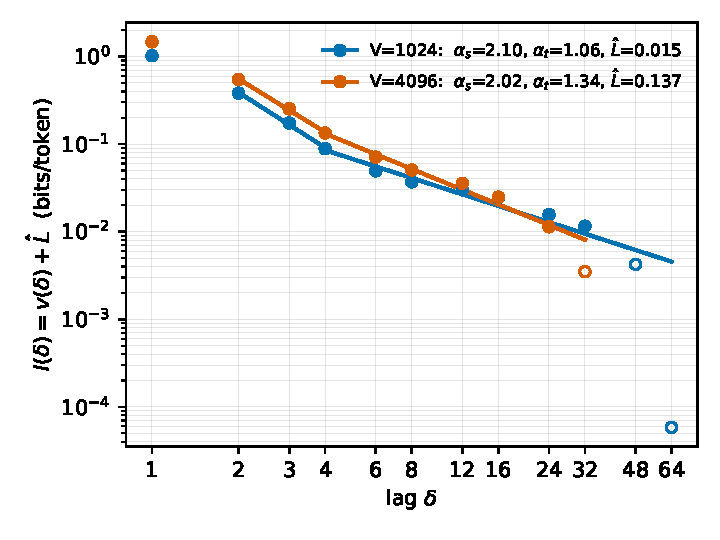
\includegraphics[width=0.72\textwidth]{lag_profile.pdf}
\caption{Corrected distance profiles $I(\delta) = v(\delta) + \hat L$
  at both scales on log-log axes (V=1{,}024 merged over both runs),
  with the two-regime fits: short-range slope $\alpha_s$ fit on
  $2 \le \delta \le 4$, tail slope $\alpha_t$ and offset $\hat L$ fit
  on $\delta \ge 4$.  Lag-1 points shown but excluded from fits; open
  circles mark corrected values below twice the fit residual
  (consistent with zero).  The break at $\delta \approx 4$ separates
  the two regimes.}
\label{fig:lag-profile}
\end{figure}

\section{Comparison with published results}
\label{sec:comparison}

\paragraph{Units.}
Every number in this paper is in bits per \emph{token}, computed by a
single sequential pass over the whole corpus.  The compression
literature reports bits per \emph{character} (bpc) on the raw file.
\texttt{text8} contains $100{,}000{,}000$ characters and
$17{,}005{,}207$ tokens, so one token accounts on average for
$5.8806$ characters (its letters plus the following space).  Dividing
bits per token by $5.8806$ therefore converts our numbers to bits per
character.  The conversion alone does not make the numbers
comparable, for the reason spelled out next.

\paragraph{What our codes encode and what they leave out.}
All experiments in this paper run on a \emph{reduced} stream: every
token outside the $K$ most frequent is replaced by the single symbol
$\langle\mathrm{unk}\rangle$.  Our codelength is the number of bits
needed to transmit this reduced sequence.  A decoder receiving it
recovers the exact sequence of frequent words, but at each position
holding an $\langle\mathrm{unk}\rangle$ it learns only \emph{that} a
rare word occurred there --- not which one.  The original file cannot
be reconstructed from what we transmit.  At $V=1{,}024$ this affects
$32.5\%$ of all tokens (average length $8.14$ characters including
the trailing space); at $V=4{,}096$, $18.0\%$ ($8.37$ characters).
The published figures below, in contrast, are for programs whose
output reconstructs the file byte for byte.  To compare, we must
additionally encode the spelling of every rare word.  Because
\texttt{text8} is exactly its tokens joined by single spaces, a
token-level code plus a character-level code for the rare words
reconstructs the file exactly; the cost of the character-level part
is estimated below.

\paragraph{Published reference points and their rules.}
(i) \emph{Mahoney's Large Text Compression Benchmark} ranks programs
on \texttt{enwik8} and \texttt{enwik9}, the raw Wikipedia dumps;
\texttt{text8} is the cleaned, lower-cased first $10^8$ bytes of
\texttt{enwik9} and was created by Mahoney as the small test file for
this benchmark.  The ranking criterion is the compressed size
\emph{plus the size of the zipped decompressor}; the program makes
one pass over the file, and everything the decoder needs is counted;
time and memory are reported but not limited.  This matches our
setting: our decoder needs the algorithm and a handful of parameters,
of negligible size.  Mahoney's test-data page lists results on
\texttt{text8} itself: \texttt{gzip} $33{,}048{,}240$ bytes $= 2.64$
bpc; \texttt{bzip2} $26{,}395{,}400$ bytes $= 2.11$ bpc;
\texttt{ppmd} $20{,}029{,}751$ bytes $= 1.60$ bpc; \texttt{paq8h}
$17{,}461{,}782$ bytes $= 1.40$ bpc.  The strongest current program
of this kind, \texttt{cmix}, compresses \texttt{enwik8} (same length,
but with markup and mixed case) to $14{,}623{,}723$ bytes $= 1.17$
bpc.
(ii) \emph{The Hutter Prize} is a standing competition on
\texttt{enwik9} only.  The deliverable is a self-extracting archive;
the measured quantity is its total size, decompressor included.  The
record is $114{,}156{,}155$ bytes $= 0.913$ bpc (2023, a \texttt{cmix}
derivative).  Constraints: a single machine, less than $10$\,GB of
RAM, less than $50$ hours of running time, and a minimum improvement
of $1\%$ over the record, paid at about $5{,}000$\,\texteuro\ per
percent.
(iii) \emph{Neural character-level models} are evaluated differently:
\texttt{text8} is split into $90$M/$5$M/$5$M characters for
training, validation, and test; the model is trained on the training
portion with as many passes as desired; the reported number is the
bits per character the trained model assigns to the test portion.
The cost of training is not part of the reported number, so it is not
the length of any code for the file, and it is smaller than what the
same model would attain in settings (i) or (ii).  Reported values
range from $1.19$ (mLSTM) to $1.04$ (Transformer-XL with dynamic
evaluation).  If we want a number comparable to these, we can report
the bits our sequential code assigns to the last $5\%$ of the token
stream given the first $95\%$; this is available from any of our
runs.

\paragraph{Our numbers in these units.}
Our best reduced-stream results convert as follows: the context-tree
family at $V=1{,}024$, $4.9507$ bits/token, corresponds to $0.84$
bits per character; at $V=4{,}096$, $6.6807$ bits/token corresponds
to $1.14$.  Both omit the rare-word spellings described above.  A
first estimate of the missing part: encoding the spelling of every
$\langle\mathrm{unk}\rangle$ occurrence with a character model at
$2$--$3$ bits per character costs, at $V=4{,}096$, $1.507$
unknown-characters per token $\times\, (2$--$3)$ $\approx 3.0$--$4.5$
bits/token.  The total, $9.7$--$11.2$ bits/token, corresponds to
$1.65$--$1.90$ bpc: between \texttt{bzip2} ($2.11$) and \texttt{ppmd}
($1.60$) on Mahoney's list.

\paragraph{The spelling cost, measured.}
The per-occurrence estimate above can be replaced by a measurement of
the construction we actually intend: spell each distinct word once, at
its first occurrence, and treat it afterwards as an ordinary token
(the escape mechanism of PPM, in sequential form;
\texttt{scripts/spelling\_experiment.py}).  The character sequence
this scheme transmits is the concatenation, in first-occurrence order,
of the $253{,}854$ distinct words plus a terminator each,
$2{,}237{,}382$ characters over a $27$-symbol alphabet.  Coding this
stream with the context-tree family over character contexts of depth
$\le 3$ costs $3.4312$ bits/character (fixed depths: $4.284$, $3.836$,
$3.596$, $3.454$) --- more than the $2$--$3$ assumed above, as the
stream consists of rare words, largely names and foreign words, and
the character model pays its own learning cost on only $2.2$ million
characters.  The total is $7.68$ Mbit $= 0.4514$ bits/token.  A second
term goes the other way.  The fixed-alphabet token code
(Section~\ref{sec:text8}, $d = 2^{18}$) pays, at each first
occurrence, for the identity of one \emph{specific} previously unseen
symbol; with spellings transmitted, the decoder only needs the event
``a new symbol'', and since the exchangeable mixture puts equal mass
on all unseen symbols, the saving at a first occurrence with $u$
unseen symbols is $\log_2 u$.  Summed over the corpus this is
$4.24$ Mbit $= 0.2496$ bits/token.  The net cost of full fidelity is
therefore $0.4514 - 0.2496 = 0.2018$ bits/token, and any token-level
codelength $X$ converts to a full-fidelity figure of
$(X + 0.202)/5.8806$ bits/character.  For the memoryless code,
$X = 10.895$ gives
\[
  \textbf{1.8870 bits/character},
\]
the first number in this paper that is the length of a code for the
file.  It is below \texttt{bzip2} ($2.11$) and above \texttt{ppmd}
($1.60$), and uses no memory at all.  The first-order codes at the
full vocabulary improve it twice: the complete map ($X = 10.0909$,
Section~\ref{sec:state-family-endpoints}) gives $1.7503$, and the
pooled family with its interior optimum
($X = 9.7826$, Table~\ref{tab:interior-m}) gives
\[
  \textbf{1.6979 bits/character}.
\]
The tally: $1.8870$ memoryless, $1.7503$ complete first order,
$1.6979$ pooled first order; the remaining distance to \texttt{ppmd}
is $0.098$ bpc.

\paragraph{Prospects.}
With the conversion $(X + 0.202)/5.8806$ in hand, the remaining
question is how far the token-level codelength $X$ can be reduced,
and the reference points translate into targets for $X$: matching
\texttt{ppmd} ($1.60$) requires $X = 9.21$ bits/token at the full
vocabulary; matching \texttt{paq8h} ($1.40$) requires $X = 8.03$.
For scale: the memoryless code has $X = 10.895$, and the in-sample
first-order conditional entropy of the full-vocabulary stream is
$7.286$ (Section~\ref{sec:text8}), so a first-order sequential code
beats \texttt{ppmd} if its learning cost stays below $1.9$ bits/token
and \texttt{paq8h} if it stays below $0.75$.  Both full-vocabulary
structures are now measured.  The complete first-order map misses both
thresholds (learning cost $2.805$ bits/token); the pooled family
recovers $0.31$ of that (learning cost $2.496$ over the plug-in
value, but only $M^\star$-resolution structure attempted), and the
depth-2 tree at full vocabulary adds nothing --- depth is not where
the next bits are (Table~\ref{tab:context-tree-large}).  What has NOT
yet been tried, and is the direct product of these two measurements,
is their combination: trees whose context alphabet is the pooled one
($b_{M^\star}$ applied to the history), spending depth only on the
few thousand contexts that can afford it, and pooled analogues with
several backoff tiers rather than one.  The remaining token-level
distance to \texttt{ppmd} is $9.7826 - 9.2072 = 0.575$ bits/token.  Two further reductions follow the two regimes of
Figure~\ref{fig:lag-profile}: deeper adaptive context trees for the
short-range regime ($\alpha_s \approx 2$), and the pooled lag
predictors of scheme 5 for the tail ($\alpha_t \approx 1$).  The
programs between $1.60$ and $1.1$ on Mahoney's list differ from
\texttt{ppmd} mainly in that they combine predictions from many
context sets, including non-contiguous ones, through mixing networks
whose weights are set by online gradient methods; the pooled-lag
construction computes a combination of the same kind, with weights
determined by a posterior.  Values below $1.0$ bpc appear on
\texttt{enwik9} ($0.913$) and in the neural setting ($1.04$ with
training cost excluded); neither is within reach of the constructions
in this paper as they stand.

\paragraph{Roadmap.}
The work is organized in phases; the first two are complete and,
as of this revision, \emph{verified}: every number in this paper has
been recomputed on a certified table store (moment values accurate to
$\sim 10^{-7}$ nats, checked against independent methods), and all
reruns --- including the full-vocabulary runs that previously
required a 200-GB cluster node --- now execute on a laptop, in
minutes to tens of minutes each.  \emph{Phase 0} (done): the
full-fidelity accounting --- escape mechanism, spelling model, index
correction --- giving the conversion above and the $1.8870$ bpc
memoryless figure.  \emph{Phase 1} (done): the vocabulary sweep of
the state-family and context-tree experiments up to the full
vocabulary, and the KT-leaf ablation; outcome: the interior optimum
(Table~\ref{tab:interior-m}), the $1.6979$ bpc figure, and the
finding that further gains at full vocabulary lie in pooled context
alphabets.  \emph{Phase 2} (done): the sequential pooled-lag evaluator ---
per-step predictive distributions of the layered per-state mixtures,
refreshed at checkpoints, pooled under both combination rules with
grids averaged at sequence level.  Outcome
(Section~\ref{sec:pooled-result}): the long-range tail is worth
$0.064$ bits/token over the first-order expert, and the data selects
the additive rule over the tempered product.

\emph{Stage A (text8): close the $0.575$ bits/token to
\texttt{ppmd}.}  Four measured increments: (i)~the Phase-2 result;
(ii)~the pooled-context tree --- the pooling map $b_{M^\star}$
applied to the \emph{history}, with tree depth grown on top of the
resulting affordable context alphabet, now directly at depth $3$
(the counting rewrite removed the depth barrier); (iii)~multi-tier
backoff --- nested frequency tiers in place of the single backoff
row, the natural refinement of the interior optimum; (iv)~the best
resulting structure run as a sequential code, the number comparable
to Mahoney's table.  These attack exactly the two regimes of
Figure~\ref{fig:lag-profile}; \texttt{ppmd} ($1.60$) is a realistic
target for this stage, \texttt{paq8h} ($1.40$) a possibility if the
increments stack.

\emph{Stage B (enwik8): fidelity, not modeling.}  \texttt{enwik8} is
raw wiki text --- markup, capitalization, punctuation --- so the
tokenizer and the spelling/escape model must be rebuilt on a larger
character alphabet under the same measure-every-bit discipline as
Phase 0, while the token-level machinery transfers unchanged.
Deliverable: whole-file bits/character on Mahoney's rules (the
program reproduces the file exactly; everything is paid for).

\emph{Stage C (enwik9): scale, not novelty.}  The audited per-task
plan is in the companion complexity notes: counting and the sparse
normalization are implemented; the table store builds in under two
node-hours at that scale; static models are node-hours and
sequential runs node-days on one 64-core, 256-GB node.  Reported
both as whole-file bits/character and as bits on the last $5\%$
given the first $95\%$ (comparable to neural results, whose
training-excluded numbers are otherwise not comparable).

Out of scope, deliberately: the sub-$1.1$ region of Mahoney's list.
Those programs combine hundreds of hand-designed context models
through mixing networks tuned by online gradient steps; reaching
them would abandon this paper's design principle --- posteriors over
generated families --- and is a different project.

\section{Generated state maps}
\label{sec:outlook}

State maps that summarize \emph{much longer} contexts, and the
criterion that selects among them.  Throughout, two design principles are held fixed:
(a) every predictor is a Bayesian mixture; (b) the prior over state
maps is \emph{generated} by products or recursion --- so that a broad
range of memory complexities arises implicitly, as the layered
construction does for distribution complexity --- rather than designed
explicitly.  One fact keeps everything computable: any state map
$\sigma$ that is deterministic given the past and independent of the
data leaves the successors of each state exchangeable, so per-state
layered mixtures, profile-only evaluation, and deduplication apply
unchanged, and the codes remain sequential.  Five schemes, in
increasing generality:

\begin{enumerate}
\item \emph{Recursive tree growth (context trees with layered leaves).}
  Generate $\sigma$ by a branching process: each context splits into its
  per-token refinements with probability $\tfrac12$, recursively, to
  maximal depth $D$.  This recursive coin flip defines a prior over all
  variable-length suffix state maps, and the mixture over the entire
  family is computable without enumeration by the context-tree identity
  $\beta(\mathrm{node}) = \tfrac12\, q^{\mathrm{avg}}(\mathrm{node}) +
  \tfrac12 \prod_{\mathrm{children}} \beta(\mathrm{child})$, evaluated
  bottom-up --- context-tree weighting with the layered mixture in place
  of KT at every node (the layered prior dominates KT on large
  alphabets \cite{layered2026}).  The growth process
  is to state maps what coordinatewise multiplication is to
  distributions.  (Implemented and running; see
  Section~\ref{sec:context-tree}.)
\item \emph{Random recursive automata (reservoir states).}  To reach
  beyond bounded suffixes: $s_t = h(s_{t-1}, x_t)$ with $h$ a
  \emph{random} transition function on $S$ states --- a state that can
  depend on the entire past.  The prior is the randomness of $h$ (the
  architecture-as-prior view of \cite{layered2026} in its purest form);
  the complexity parameter is $S$, and a mixture over an ensemble of
  sizes covers a range of complexities at negligible cost.  The scheme
  measures what an undesigned recursive summary captures per state,
  compared with suffix states at equal $S$.
\item \emph{Learned coarsenings (approximate causal states).}  Merge
  (state, token) pairs with similar continuation statistics --- an
  information-bottleneck construction.  Here $\sigma$ depends on the
  data, so the code must be made sequential again: either two-part
  (transmit the merge structure at its description cost) or causal
  (cluster on a prefix, apply to the remainder).  Comparing it with
  schemes 1--2 measures the value of designing states over generating
  them.
\item \emph{Composed random coarsenings (the layered construction for
  memory itself).}  $\sigma = \varphi_R \circ \cdots \circ \varphi_1$
  with each $\varphi_r$ a random elementary coarse-graining of (state
  $\times$ token); the composition depth $R$ is the memory analogue of
  the emission depth $L$.  By the mechanism that makes products of
  simplex draws spread their spectra, composition of random maps should
  spread the effective memory of typical draws, so that averaging over
  $R$ yields one prior covering all memory complexities at logarithmic
  cost.  Scheme 2 is the $R=1$ special case.  Compositions of random maps are
  analyzable, so this is the candidate for deriving --- not merely
  fitting --- the regret spectrum and scaling laws of memory.
\item \emph{Pooled lag experts (combining predictions, not states).}
  Every scheme above combines memories by \emph{refining the state
  partition}, and Table~\ref{tab:product-family-4096} shows the price:
  refinement multiplies the number of states, so the learning cost
  grows multiplicatively.  The complementary move is to combine
  \emph{predictions}.  Each lag $\delta$ defines a state map
  $\sigma^{(\delta)}: s_t = x_{t-\delta}$ --- deterministic and
  data-independent, so the machinery of this paper applies unchanged,
  at cost \emph{additive} in the number of lags ($\Delta \cdot V$
  states, not $V^\Delta$).  The question is how to combine the per-lag
  estimates $p_\delta(x \,|\, x_{t-\delta})$ into one predictive
  distribution; three combinations of increasing strength follow.
  (a) The Bayesian mixture over $\delta$
  (eq.~\eqref{eq:state-average} again) adds no cost and remains
  sequential, but can only \emph{select}; its posterior measures the
  value of each lag.  With pairwise information only and
  tractability constraints this is also what the optimal (Chow--Liu)
  tree structure degenerates to: attach $x_t$ to its single best lag by
  mutual information.  (b) Under the (naive-Bayes) assumption that the
  past tokens are conditionally independent given $x_t$, Bayes' rule
  gives the logarithmic pool
  \[
    q\bigl(x \,\big|\, \{x_{t-\delta}\}\bigr) \;\propto\;
    p(x) \prod_{\delta}
    \frac{p_\delta(x \,|\, x_{t-\delta})}{p(x)},
    \qquad\text{i.e.}\quad
    \log q = \log p(x)
    + \sum_\delta \mathrm{PMI}(x;\, x_{t-\delta}) + \mathrm{const}:
  \]
  each lag contributes its pointwise mutual information with the
  candidate token and the prior is counted once.  Unlike a mixture, the
  product \emph{accumulates} evidence: two weak experts that agree
  yield a confident prediction, which no mixture can produce.  Its
  failure mode is double counting when lags are redundant, and in text
  they are (Table~\ref{tab:lag-family}, item (iii)).  (c) The
  correction is the
  maximum-entropy joint consistent with all known pairwise marginals
  \emph{including those among the conditioning variables} --- a pairwise
  Markov random field $q(x \,|\, \cdot) \propto
  \exp\bigl(\sum_\delta \lambda_\delta(x, x_{t-\delta})\bigr)$, of
  which (b) is the special case of mutually independent lags.  Its
  cheap surrogate is the weighted pool
  $q \propto p(x)^{1-\sum_\delta w_\delta} \prod_\delta
  p_\delta(x \,|\, x_{t-\delta})^{w_\delta}$, where $w_\delta = 1$
  recovers (b) and $w_\delta < 1$ discounts redundancy.  In our
  framework the weights are not computed from a dependence analysis but
  \emph{learned}: a prior over $w$, mixed online, possibly with
  different weights in different contexts, at the usual
  $(\log_2|\mathrm{grid}|)/n$ price.  Recursion --- pool lags $1,2$
  into one expert, lags $3,4$ into another, then pool the pools over
  doubling distance bands --- reaches distance $2^R$ at cost linear in
  $R$.  Two limits apply.  First, pooling needs per-step predictive
  distributions and per-step normalization, so its implementation
  requires the sequential machinery deferred in
  Appendix~\ref{sec:pairs}.  Second, pairwise probabilities cannot
  detect \emph{synergy}: for a source in which $x_t$ is a function of
  $(x_{t-1}, x_{t-2})$ jointly but independent of each alone, every
  pairwise conditional is flat and no pooling, however weighted, can
  predict; only combined states (schemes 1 and 4, or the product
  grids) capture such structure.  Pooling and state refinement are
  therefore complements: pooling captures the \emph{additive} part of
  the past at linear cost, while state refinement, at multiplicative
  cost, is the only way to capture the \emph{synergistic} part.  In
  these terms, the $57$ split contexts of Table~\ref{tab:context-tree}
  are where the synergistic part is concentrated.  The construction
  parallels attention in neural networks, where heads read tokens at
  several offsets and combine them with content-dependent weights.
  (Combination (a) is implemented and measured; see
  Section~\ref{sec:lag-family}.)
\end{enumerate}

\paragraph{Ultimate goal.}
The ideal, not directly learnable, is the minimal sufficient statistic
of the past
(causal states: two pasts equivalent iff they induce the same law of the
future).  The operational goal is the lift of \cite{layered2026} from
i.i.d.\ sources to sources with memory: a single coherent Bayesian
predictor, generated by layered and recursive randomness rather than
designed priors, whose prior mass spans predictors of all joint (memory
$\times$ distribution) complexities --- so that every source is charged
roughly its own complexity, with regret governed by identifiable
discovery rates and scaling laws that can be derived.  An exactly
solvable instance of architectures-as-priors in which \emph{recurrence},
not only depth, is part of the architecture; two nested layered
constructions, one spreading emission complexity ($L$), one spreading
memory complexity ($R$), each averaged, each priced, jointly adapting.


\appendix

\section{The joint-pair diagnostic}
\label{sec:pairs}

This appendix records the first memory experiment: an in-sample
diagnostic of the depth-averaged \emph{joint} estimator on
sliding-window pairs.  It is referenced from
Section~\ref{sec:states} as the measured evidence for what coupling
the rows of a conditional through one joint prior buys.  The symbol is
the \texttt{text8} word alphabet defined at the start of
Section~\ref{sec:states}.  We describe exactly what \texttt{scripts/pair\_experiment.py}
computes.

\paragraph{Vocabulary sequence.}
To scale from laptop to cluster we reduce the vocabulary to the $K$ most
frequent tokens plus a single $\langle\mathrm{unk}\rangle$ bucket
($V=K+1$ symbols; the structure of the order-one partition of
\cite{layered2026}, Section~5.4).  All quantities below refer to the
\emph{reduced} token stream $x_1,\dots,x_n$; the pair alphabet is
$d=V^2$, and $L_{\max}=\operatorname{round}(2\cstar\ln d)$ as always.  The
targets are the empirical entropies of the same reduced stream: the unigram
entropy $\hat H_1$ and the conditional entropy
$\hat H(x_{t+1}\,|\,x_t)=\hat H_{\text{pair}}-\hat H_{\text{first}}$, both
in-sample.

\paragraph{Estimate.}
The joint distribution of pairs is estimated \emph{in-sample}
(plug-in): the entire multiset of $n-1$ sliding pairs, with count profile
$\lambda$, informs the estimate, and the log-loss is evaluated on the same
sequence.  The estimate is the depth-averaged mixture's posterior mean.
For a pair currently at count $c$ (including $c=0$ for unobserved pairs),
\begin{equation}
\label{eq:predictive}
  \hat p(c) \;=\; \sum_{L=1}^{L_{\max}} w_L\, p_L(c),
  \qquad
  w_L \;=\; \frac{q_L(\lambda)}{\sum_{L'} q_{L'}(\lambda)},
  \qquad
  p_L(c) \;=\; \frac{q_L(\lambda + e_c)}{q_L(\lambda)},
\end{equation}
where $\lambda+e_c$ moves one symbol from count class $c$ to $c+1$.  The
ratio $p_L(c)$ is not evaluated by two independent profile computations;
at a saddle $u^\star$ of the outer integral the posterior mean of a
coordinate with count $c$ is
\[
  p_L(c) \;\approx\; \frac{\rho_L(c, u^\star)}{N},
  \qquad
  \rho_L(c,u) = e^{u}\,\frac{\phi^{(L)}_{c+1}(e^u)}{\phi^{(L)}_{c}(e^u)},
\]
with $\phi^{(L)}_r$ the layer-recursion moment functions of
\cite{layered2026}, Appendix~B.  The saddle equation
$\sum_i \rho_L(c_i,u^\star)=N$ makes the class-weighted sum of these
predictive masses normalize \emph{exactly} at saddle order; when the
integrand has several significant peaks (deep layers with heavy counts)
the peaks are combined with their scan weights.  $p_L(1)$ is exact add-one
at $L=1$.  A final numerical renormalization absorbs the residual
$O(1/N)$-level error, which the program reports as a diagnostic
(validated against exact ratio computations to $<2\%$ per depth in the
test suite; the aggregate normalization error is far smaller).

\paragraph{Conditionals and score.}
Conditional probabilities come from row normalization,
$\hat p(b\,|\,a) = \hat p\bigl(c_{ab}\bigr) / \sum_{b'} \hat
p\bigl(c_{ab'}\bigr)$, with unobserved successors carrying the class-$0$
mass; the row sums reduce to per-row count histograms.  The score is the
in-sample conditional log-loss
\[
  \ell \;=\; -\frac{1}{n-1}\sum_{t=2}^{n} \log_2 \hat p(x_t \,|\, x_{t-1})
  \;=\; -\frac{1}{n-1}\sum_{a,b} m_{ab}\, \log_2 \hat p(b\,|\,a),
\]
compared like-for-like with the in-sample $\hat H(x_{t+1}|x_t)$; the gap
$\ell - \hat H(x_{t+1}|x_t)$ is the estimator's smoothing-plus-discovery
cost.  This plug-in scheme is a diagnostic, not a code: fully sequential
(decodable) variants --- the per-state construction of
\cite{layered2026}~Section~5.4, and the causal joint-conditional predictor
with checkpointed refreshes --- are deferred to a later stage.

\begin{table}[ht]
\centering
\begin{tabular}{rrrrrrrr}
\toprule
$K$ & $d=V^2$ & $L_{\max}$ & pairs obs. & $\hat H_1$ & $\hat H(x'|x)$ & $\ell$ (plug-in) & gap \\
\midrule
    63 & $2^{12}$ & 39 &      3{,}762 & 3.224 & 2.733 & 2.7334 & 0.00001 \\
   255 & $2^{16}$ & 52 &     45{,}076 & 4.423 & 3.709 & 3.7098 & 0.00055 \\
 1{,}023 & $2^{20}$ & 66 &    307{,}076 & 6.063 & 4.979 & 4.9878 & 0.00850 \\
 4{,}095 & $2^{24}$ & 79 & 1{,}172{,}941 & 8.051 & 6.338 & 6.3951 & 0.05747 \\
16{,}383 & $2^{28}$ & 92 & 2{,}578{,}046 & 9.702 & 7.154 & 7.3104 & 0.15624 \\
\bottomrule
\end{tabular}
\caption{Pair experiment on full \texttt{text8} ($n = 17{,}005{,}207$
  tokens, $n-1$ sliding pairs), vocabulary reduced to the top $K$ tokens
  plus $\langle\mathrm{unk}\rangle$.  Empirical (in-sample) unigram and
  conditional entropies of the reduced stream in bits/token, the plug-in
  conditional log-loss $\ell$ of the depth-averaged joint estimate, and
  the gap $\ell-\hat H(x'|x)$.  At the first two rungs the pair alphabet
  is densely observed ($\approx 4{,}150$ and $260$ samples per possible
  pair) and the plug-in estimate sits essentially on the ceiling, with the
  joint posterior a point mass at $L=7$ resp.\ $L=6$
  ($\approx 0.5$--$0.8\,\ln d$); the sparsely observed regime begins at
  $K = 1{,}023$ ($\le 16$ samples per possible pair, $71\%$ of the pair
  alphabet unseen), where the gap opens but remains small:
  $0.0085$ bits/token, i.e.\ $0.17\%$ of the conditional entropy, with
  the joint posterior again a point mass ($L=8$).  The sequence of gaps
  ($1.3\cdot10^{-5} \to 5.5\cdot10^{-4} \to 8.5\cdot10^{-3} \to
  5.7\cdot10^{-2} \to 1.56\cdot10^{-1}$) measures the discovery cost that
  made the earlier full-vocabulary attempt impractical; its growth
  factors from one row to the next decrease ($\times 42 \to \times 15
  \to \times 6.8 \to \times 2.7$).  Even at $K=16{,}383$, with $99\%$ of
  the $2^{28}$ pair alphabet unseen and $6.6$ samples per observed pair,
  the gap is $2.2\%$ of the conditional entropy.  The joint posterior
  remains a point mass throughout, at depths $L = 7, 6, 8, 10, 15$ that
  grow as the pair distribution becomes sparse relative to its alphabet
  --- the mirror image of the drift reported in
  Section~\ref{sec:text8}, where the posterior moved to shallow depths
  as \texttt{text8}'s alphabet filled up.  Predictive normalization
  diagnostics: $10^{-13}$--$10^{-6}$ in all rows.}
\label{tab:pairs}
\end{table}


\end{document}
